\documentclass{article}
\usepackage[utf8]{luainputenc}
\usepackage[T1]{fontenc}
%\usepackage[a4paper,margin=0.75in, bottom=1in]{geometry}
\usepackage{fullpage}
\usepackage{listings}
\usepackage{courier}
\usepackage{amsmath}
\usepackage{amssymb}
\usepackage{enumerate}
\usepackage{graphicx}
\usepackage{hyperref}

\begin{document}
	
	\setlength{\parindent}{0em} 
	
	\hrulefill
	\begin{center}
		\bfseries % Fettdruck einschalten
		\sffamily % Serifenlose Schrift
		\begin{huge}
			GTI: Grundlagen der Theoretischen Informatik
		\end{huge}\\
		\begin{Large}
			Sommersemester 2017, 8. Übungsblatt
		\end{Large}\\
		\begin{small}
			Valentin Wolf, Luis Herrmann; Tutor: Kristin Knorr; Mo 12:00-14:00
		\end{small}
		
		\vspace{-10pt}
	\end{center}
	\hrulefill
	
\section*{Aufgabe 1 - \textit{Nicht nach links!}}
\begin{enumerate}[a)]
	\item Wir betrachten eine deterministische 1-Band-1-Kopf TM, die die Sprache entscheidet und nur $R$, $N$ benutzt. Diese kann durch eine dfa simuliert werden. Das zeigen wir wie folgt: Nehmen wir an, die TM bewegt sich beim lesen eines Wort $w \in \Sigma^*$ nunächst nur nach rechts $R$ und macht im $n$-ten Schritt die Bewegung $N$. Dann verhält sich die TM bis zu diesem Schritt wie ein dfa mit der Übergangsfunktion $\tilde{\delta}$:
	\begin{equation}
		\forall 0 \le i < n : \tilde{\delta}(q_i, w_{i+1}) = q_{i+1} \quad \text{ für } \quad \delta(q_i, w_{i+1}) = (q_{i+1},a\in \Sigma,R)
	\end{equation}
	
	wobei die $q_i \in Q$ sind und insbesondere zwei $q_i$ identisch sein können. Welches Zeichen $a$ zurückgeschriben wird ist dabei unerheblich, da sich der Kopf nicht wieder nach links bewegen kann, um dieses zu lesen. Nehmen wir an, der Kopf der TM macht in den nächsten $m-1$ Schritten zunächst die Bewegung $N$ und dann eine Bewegung $R$, also:
	\begin{equation}
		\forall 0 \le j < m: \delta(q_{n+j}, a_j) = (q_{n+j+1}, a_{j+1}, N)
	\end{equation}
	
	 Mit $a_0 := w_n$. Offenbar muss die TM irgendwann eine Bewegung nach rechts durchführen und liest dann $w_{n+1}$. Denn nach spätestens $|Q||\Gamma|$ Schritten würde die TM sonst in eine Schleife geraten und würde nicht terminieren. Dann würde die TM aber nicht die Sprache $L$ entscheiden.
	 
	 In der Simulation mit dem dfa überspringen wir also alle Schritte, in denen die Bewegung $N$ erfolgt, außer es wird ein Endzustand erreicht.
	 \begin{equation}
	 	\tilde{\delta}(q_n,a) = q_{n+m} \text{ mit } \delta(q_{n+m-1}, a_{m-1}) = (q_{n+m},a_m,R)
	 \end{equation}
	 
	 Indem wir dies für alle Übergänge der TM Maschine tun, haben wir gerade einen simulierenden dfa beschrieben und sind fertig.
	 
	\item Wir wollen $L :=  \{a^n b^n c^n | n \ge ^1\}$ mithilfe einer 1-Band-2-Kopf-TM entscheiden. Da wir eine Zweikopf-TM betrachten, hat die Übergangsfunktion die Form $\delta : Q \times \Sigma^2 \to Q\times \sigma^2 \times \{R,N\}^2$.
	
	Die Idee zur Kostruktion ist nun Folgende:
	\begin{enumerate}[(1.)]
		\item Bewege 1. und 2. Kopf nach rechts über das erste Zeichen des Eingabewortes. Falls von den Köpfen ein blank oder ein bel. Zeichen $\neq a$ gelesen wird, verwerfe.
		\item Bewege 1. Kopf nach rechts, solange $(a,a)$ gelesen wird. Falls $(a,b)$ gelesen wird, gehe über zu Schritt (3.). Falls der 2. Kopf ein Zeichen ungleich $a$, $b$ liest, verwerfe Eingabe.
		\item Bewege beide Köpfe nach rechts, solange $(a,b)$ gelesen wird. Falls $(b,c)$ gelesen wird, gehe über zu Schritt (4.). Falls etwas außer $(a,b)$, oder $(b,c)$ gelesen wird, verwerfe.
		\item Bewege beide Köpfe nach rechts, solange $(b,c)$ gelesen wird. Falls $(c,\text{\textvisiblespace})$ gelesen wird, akzeptiere. Falls etwas außer $(b,c)$, oder $(c,)$ gelesen wird, verwerfe.
	\end{enumerate}
	Wenn die TM akzeptiert, muss die Anzahl der $a$'s denen der $b$'s gleich sind und ferner die Anzahl der $b$'s denen der $c$'s gleich sein, also muss das Wort dann die Form $a^n b^n c^n$ für ein geeignetes $n \ge 1$ haben.
	
	Wir geben noch eine explizite TM an:
	
	\begin{minipage}{\textwidth}
		\centering 	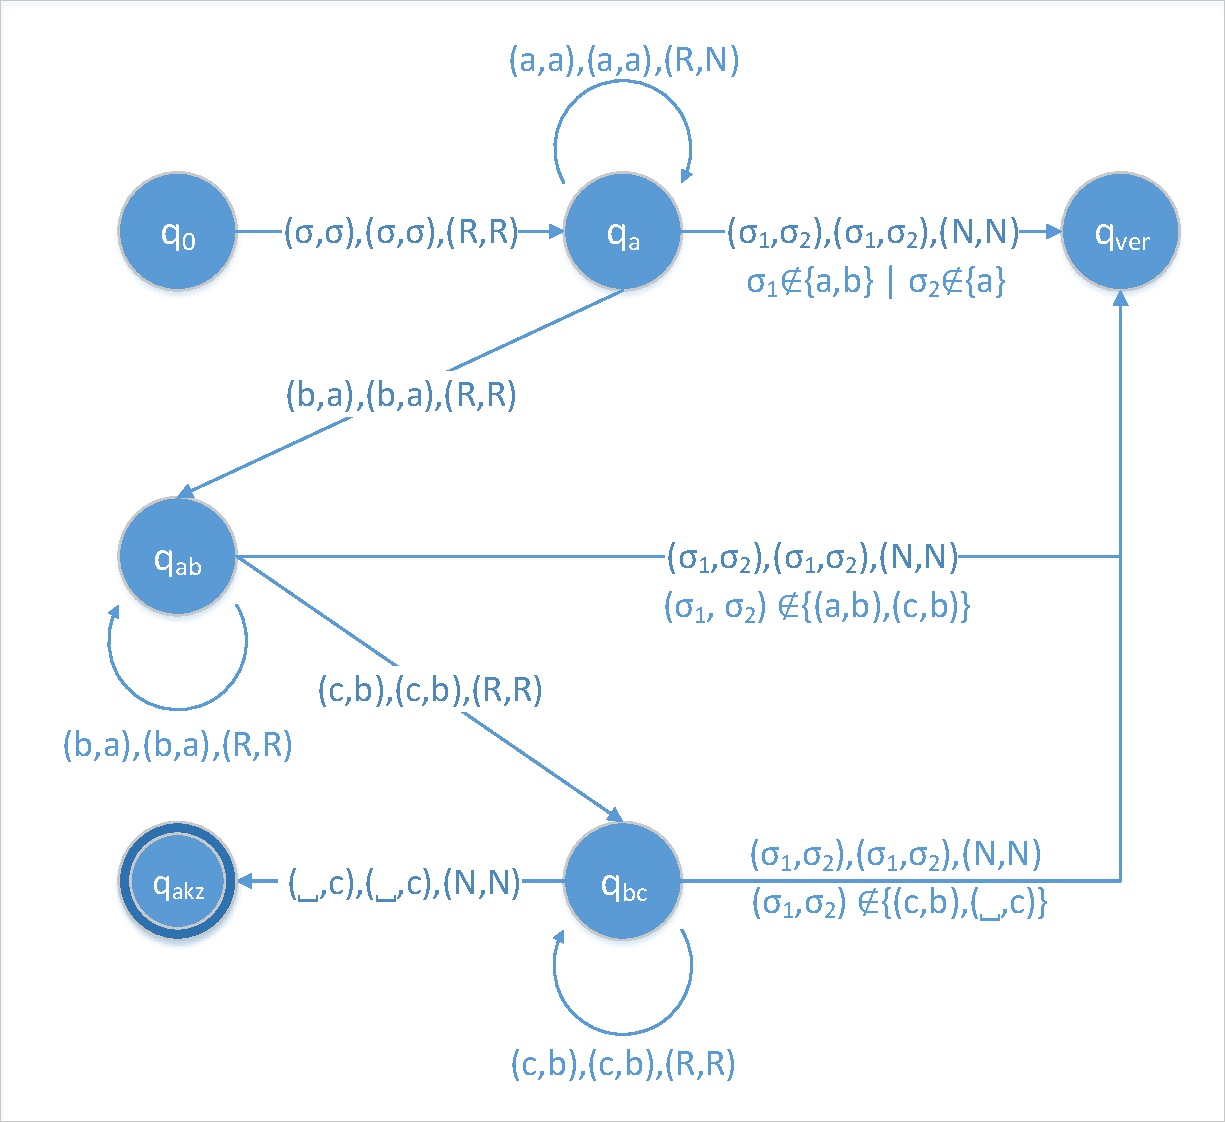
\includegraphics[width=0.75\textwidth,page=1,trim={2 2 2 4},clip]{diagramme.pdf}
	\end{minipage}
	
	Offenbar terminiert die TM für alle Eingabewörter und somit ist die Sprache entscheidbar. Die Schreibfunktion wird nicht benötigt, da immer nur bereits gelesene Zeichen auf das Band zurückgeschrieben werden.
	
\end{enumerate}

\section*{Aufgabe 2 - \textit{Regulär I}}

Sei $L$ reguläre Sprache über $\Sigma$ und $w\in\Sigma^*$. Wir zeigen, dass die Sprache $L_w = \{v\in L | v \text{enthält } w \text{ als Teilstring}\}$ auch regulär ist.\\

Betrachten wir zunächst einen dfa $A = (Q_w, \Sigma, q_0, \delta_w, F_w)$, der die Sprache $L_w = \{w\}$ akzeptiert. Wir konstruieren diesen wie folgt: $Q = \{q_0,q_1,...,q_{|w|}, q_{|w|+1}\}$, $F= \{q_{|w|}\}$ und die Überführungsfunktion arbeitet wie folgt:
\begin{equation}
	\delta_w(q_i, a) = \begin{cases}
	q_{i+1},& a = w_{i+1}\\
	q_{|w| + 1}, &a \neq w_{i+1}
	\end{cases}
\end{equation}


Dann können wir mit Hilfe von $A$ einen nfa $N = (Q,\Sigma,q_0,\delta,F)$ definieren, der alle Wörter mit einem Teilwort $w$ akzeptiert, und zwar wie folgt:

\begin{minipage}{\textwidth}
	\centering \includegraphics[width=0.75\textwidth,page=2,trim={2 2 2 4},clip]{diagramme.pdf}
\end{minipage}

Oder formaler:
\begin{equation}
	\delta(q_i,a) = \begin{cases}
	\{q_0,q_1\}, &i = 0, a = w_1\\
	\{q_0\}, &i=0, a \neq w_1\\
	\{\delta(q_i,a)\}, & 0 < i < |w|\\
	\{q_{|w|}\}, & i = |w|
	\end{cases}
\end{equation}

Im akzeptierenden Zustand können wir nur landen, wenn ab irgendeiner Position von $v$ eine Sequenz von Zeichen aus dem Alphabet auftaucht, die gerade $w$ ist. Wird ein akzeptierender Zustand erst einmal erreicht (also ein Teilwort $w$ gefunden), verbleibt man in diesem bis zum Ende der Berechnung, sodass $v$ akzeptiert wird, da es unerheblich ist, wie das Rest des Wortes aussieht.\\

Es bleibt noch zu prüfen, ob das Eingabewort $v \in L$ ist. Da wir voraussetzen, dass $L$ eine reguläre Sprache, ex. hierfür ein dfa $A$ und wir können den dfa $A$ und den nfa $N$ parallel schalten und genau dann akzeptieren, wenn beide Automaten akzeptieren. Der resultierende nfa akzeptiert gerade die Sprache $L_w$ und lässt sich durch einen dfa simulieren, also ist $L_w$ regulär.

\section*{Aufgabe 3 - \textit{Regulär II}}
Sei $\Sigma = \{a,b\}$ und $L$ die Menge aller nichtleeren Wörter über $\Sigma$, deren letztes Zeichen mindestens noch einmal im Wort vorkommmt.
\begin{enumerate}[a)]
	\item Die Sprache kann durch folgenden regulären Ausdruck charakterisiert werden.
	\begin{equation}
		\alpha(L) = (\{a \cup b\}^* a \{a \cup b\}^* a ) \cup (\{a \cup b\}^* b \{a \cup b\}^* b )
	\end{equation}
	\item Die Sprache wir durch den nfa $N = (Q, \Sigma, q_0, \delta, F)$ mit $Q := \{q_0, q_a, q_b, q_{a*a}, q_{b*b}\}$ und $F := \{q_{a*a},, q_{b*b}\}$ entschieden:
	
	\begin{minipage}{\textwidth}
		\centering\includegraphics[width=0.5\textwidth,page=3,trim={2 2 2 4},clip]{diagramme.pdf}
	\end{minipage}
	
	\item Wir suchen eine Typ-3-Grammatik, sodass $L(G) = L$. Zur Erinnerung: Eine Grammatik $G = (V, \Sigma, P, S)$ ist vom Typ 3 (regulär), falls $\forall (w_1,w_2) \in P: w_1 \in V \land w_2 \in \Sigma \cup \Sigma \circ V$.
	
	Wir wählen $V = \{S,A,B,X\}$ und:
	\begin{align}
		&S \to aA | bB | X && A \to aA | bA | a  &&& B \to aB | bB | b  &&&&  X \to aX | bX | aA | bB
	\end{align}
\end{enumerate}

\section*{Aufgabe 4 - \textit{Kontextfrei}}

Sei $L$ die Sprache aller Wörter über $\Sigma = \{0,1\}$, die genau eine 1 mehr als 0 hat. Wir suchen eine kontextfreie Grammatik, die $L$ erzeugt. Zur Erinnerung: $G$ heißt kontextfrei, falls $\forall (w_1,w_2) \in P: w_1 \in V \land 1 \le |w_2|$.

Wir wählen $V = \{S,X\}$ und:
\begin{align}
	& S \to 1 | 1X | X1 | X1X && X \to 01 | 10 | 0X1 | 1X0 | XX
\end{align}

Die Konstruktion ist derart, dass $X \overset{*}{\to}$ Wort mit gleichvielen 0en und 1en. Logischerweise muss $S \overset{*}{\to}$ Wort mit genau einer 1 mehr als 0en. Die Regeln für die Variable $S$ entsprechen dabei der Position der zusätzlichen 1 in einem anderen Wort.

Wir beweisen die Richtigkeit der Grammatik induktiv.

\subsubsection*{I.A.:}

$n=1$: $X \to 01 | 10$\\
$n=2$: $X \to XX \to 0101 | 0110 | 1001 | 1010$, $X \to 1X0 \to 1100$, $X \to 0X1 \to 0011$

\subsubsection*{I.S.:}
\begin{enumerate}
	\item $X \overset{*}{\to} w = 0v0$
	
	$X \overset{*}{\to} w \Leftrightarrow X \to XX \to 0X110 | 011X0 | 0X11X0 \overset{*}{\to} 0x110 | 011y0 | 1z_011z_20$ oder $X \to XX \to XXX \to 0X1X1X0 \overset{*}{\to} 0u_1 1 u_2 1 u_3 0$ $\Leftrightarrow X \overset{*}{\to} x | y | z_1 | z_2 | u_1 | u_2 | u_3$. Das ist nach I.V. gewährleistet und wir haben alle möglichen Formen von Wörtern mit gleicher Anzahl von 0en wie 1en, die auf 1 anfangen und enden, abgedeckt.
	
	\item $X \overset{*}{\to} w = 0v1$
	
	$X \overset{*}{\to} w \Leftrightarrow X \to 0X1 \Leftrightarrow X \overset{*}{\to} v$ mit $|v| = |w| - 2$. Das ist nach I.V. gewährleistet.
	
	\item $X \overset{*}{\to} w = 1v0$
	
	$X \overset{*}{\to} w \Leftrightarrow X \to 1X0 \Leftrightarrow X \overset{*}{\to} v$ mit $|v| = |w| - 2$. Das ist nach I.V. gewährleistet.
	
	\item $X \overset{*}{\to} w = 1v1$
	
	$X \overset{*}{\to} w \Leftrightarrow X \to XX \to 1X001 | 100X1 | 1X00X1 \overset{*}{\to} 1x001 | 100y1 | 1z_100z_21$ oder $X \to XX \to XXX \to 1X0X0X1 \overset{*}{\to} 1u_1 0 u_2 0 u_3 1$ $\Leftrightarrow X \overset{*}{\to} x | y | z_1 | z_2 | u_1 | u_2 | u_3$. Das ist nach I.V. gewährleistet und wir haben alle möglichen Formen von Wörtern mit gleicher Anzahl von 0en wie 1en, die auf 1 anfangen und enden, abgedeckt.
\end{enumerate}

Zuletzt zeigen wir noch Nichtregularität von $L$. Angenommen, die Sprche ist regulär. Nach Pumping-Lemma existiert für $\forall z \in L$ eine Zerlegung $z = uvw$ mit $|uv| \le n, |v| \ge 1 \forall i\ge 1 : uv^i w \in L$. Betrachte das Wort $z = 1^{n+1} 0^n$. Offenbar ist $z \in L$, aber für jede Zerlegung gilt $|uv| \le n \Rightarrow uv = 1^{|uv|}$ und somit:
\begin{equation}
	uv^iw = 1^{|u|} 1^{|v|i} 1^{n+1-|uv|} 0^n = 1^{n+1 + |v|(i-1)} 0^n
\end{equation}
Da $\forall i > 1 : |v|(i-1) + n+1 > n+1$ folgt $\forall i > 1: uv^i w \not\in L$ im Widerspruch zur Annahme.

\end{document}